%
% Report -- Compact Verilog-A pn junction photodiode model
%
% Copyright (C) 2008 Mike Brinson <mbrin72043@yahoo.co.uk>
%
% Permission is granted to copy, distribute and/or modify this document
% under the terms of the GNU Free Documentation License, Version 1.1
% or any later version published by the Free Software Foundation.
%

% redefine subfigure caption
\renewcommand{\thesubfigure}{\thefigure(\alph{subfigure})}
\makeatletter
  \renewcommand{\@thesubfigure}{\thesubfigure:\space}
  \renewcommand{\p@subfigure}{}
\makeatother

% redefine subtable caption
\renewcommand{\thesubtable}{\thetable(\alph{subtable})} 
\makeatletter
  \renewcommand{\@thesubtable}{\thesubtable:\space}
  \renewcommand{\p@subtable}{}
\makeatother

\tutsection{Introduction}
Optoelectronic devices are not included in Qucs version 0.0.14 or
earlier releases of the software. With the growing importance of these
devices, and indeed the fact that they are present in an increasing
number of electronic systems, this is a significant omission. This
report presents the structure and physical details of a Qucs
implementation of a pn junction photodiode model. The photodiode model
is the first in a planned series of Verilog-a compact device models
for optoelectronic components. The report also introduces the concept
of a light bus and shows how light paths can be added to Qucs
simulation schematics. A number of example schematics are also
included in the report to demonstrate the performance of the new
Verilog-A pn junction photodiode model. The background to the work
outlined in this report was first published in the International
Journal of Numerical Modelling: Electronic Networks, Devices and
Fields in September 2008\footnote{Brinson M.E. and Jahn S., Qucs: A
GPL software package for circuit simulation, compact device modelling
and circuit macromodelling from DC to RF and beyond, published online,
5 September 2008,
\url{http://www3.interscience.wiley.com/journal/121397825/abstract}.}.

\tutsection{pn junction photodiode effects modelled} 
The Qucs pn junction photodiode model includes the following features:
\begin{itemize}
 \item Diode photocurrent response characteristics expressed as a function of light power and wavelength.
 \item Diode DC I-V characteristics in the forward and reverse bias regions including avalanche breakdown in  reverse bias.
 \item Diode bias dependent capacitance.
 \item Diode shunt resistance.
 \item Diode package series resistance.
 \item Device noise, including thermal, shot, flicker and quantum contributions.  
\end{itemize}

\tutsection{The Qucs pn junction photodiode model} 
The schematic capture symbol and equivalent electrical circuit for the
Qucs pn junction photodiode is shown in Fig.~\ref{fig:PD1}. In this
model the DC properties and capacitance of the photodiode are
represented by a semiconductor diode with a parallel shunt resistance
Rsh. Device lead resistance is represented by series resistance
Rseries\verb|_|area. A voltage-controlled current source models the
diode photocurrent. The gain of the controlled source is set as the
responsivity of the photodiode. The equivalent circuit shown in
Fig.~\ref{fig:PD1}(c) presents the complete photodiode model with
thermal, shot and flicker noise sources included. One interesting, and
unusual, feature of the Qucs photodiode noise model is the inclusion
of quantum shot noise, modelled by noise current source
\textit{Ilightn}. Photocurrent \textit{Ilight} is given by
\begin{equation}
 Ilight = Light \cdot Responsivity
\end{equation} 
    

where \textit{Light} is the optical signal in W and
\textit{Responsivity} is the the spectral responsivity in
A/W. Responsivity can also be written in terms of the photodiode
quantum efficiency given by.
\begin{equation}
 Responsivity = \dfrac{QE \cdot q \cdot \lambda}{h \cdot c} = \dfrac{QE_{percent} \cdot \lambda}{1.2398e5}
\end{equation}
where QE is the photodiode quantum efficiency, $\lambda$ is the light
wavelength in nm, $h$ is Plank's constant, c is the speed of light in
a vacuum, and $QE_{percent}$ is the quantum efficiency given in
percentage. In Fig.~\ref{fig:PD1} the optical signal path is shown as
a green line connected at the side of the photodiode symbol. In Qucs
simulations optical signals are modelled as voltage quantities
expressed as real numbers, even though they represent a power
quantity, and are shown on a schematic as green connecting lines
between components. This has the effect of clearly identifying optical
signal paths on a schematic, when compared to the blue lines which
indicate connecting wires characterised by conventional current and
voltage signals. Similarly, signal sources which input light to a
circuit are coloured green, see later example simulations.

\begin{figure}[ht]
  \centering
	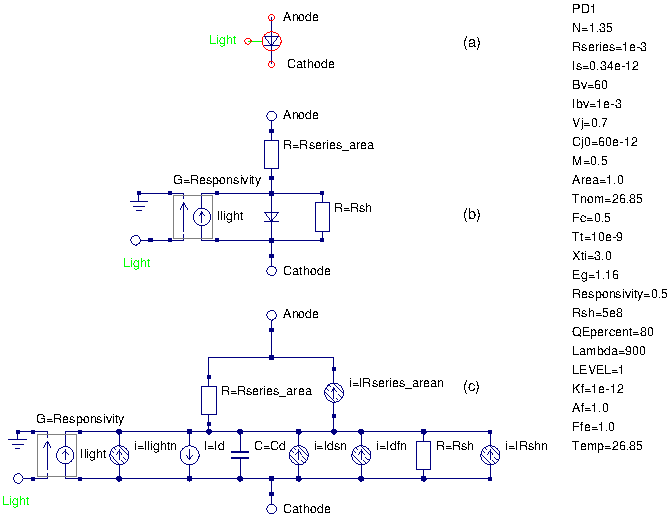
\includegraphics[width=0.7\linewidth]{PD_fig1}
        \caption{Qucs pn junction photodiode model: (a) schematic capture symbol, (b) basic model circuit, (c) full equivalent circuit, including noise }
  \label{fig:PD1}
\end{figure} 
\newpage 
\tutsubsection{Photodiode parameters}
\begin{scriptsize}
\begin{longtable}{ccllcc}
Name & Symbol & Description & Unit & Default \\
\hline
\endhead
N &  $N$ &  photodiode emission coefficient    &        &  $1.35$   \\
Rseries   & $Rseries$ & series lead resistance   & $\ohm$    & $1e-3$ \\
Is   & $Is$ & diode dark current    & A    & $0.34e-12$ \\
Bv  & $Bv$ & reverse breakdown voltage  & V  & $60.0$  \\
Ibv  & $Ns$ & current at reverse breakdown voltage    & A  & $1e-3$  \\
Vj & $Vj$ & junction potential   & V    & $0.7$  \\
Cj0  & $Cj0$ & zero bias junction capacitance   & F    & $60e-12$  \\
M  & $M$ & grading coefficient   &     & $0.5$  \\
Area  & $Area$ & diode relative area  &     & $1$  \\
Tnom & $Tnom$ & parameter measurement temperature   & \degree C    & $26.85$ \\
Fc  & $Fc$ & forward-bias depletion capacitance coefficient   &    & $0.5$  \\
Tt  & $Tt$ & transit time  & s    & $10e-9$  \\
Xti   & $Xti$ & saturation current temperature exponent   &     & $3.0$  \\
Eg & $Eg$ & energy gap  & eV    & $1.16$  \\
Responsivity  & $Responsivity$ & responsivity  & A/W     & $0.5$  \\
Rsh & $Rsh$ & shunt resistance  &  $\ohm$  & $5e8$  \\
QEpercent  & $QEpercent$ & quantum efficiency  & \%     & $80.0$  \\
Lambda  & $Lambda$ & light wavelength   & nm    & $900.0$  \\
LEVEL   &          & responsivity calculator selector$^{*}$& & $1$ \\
Kf   & $KF$  & flicker noise coefficient                &    & $1e-12$  \\
Af   & $Af$  & flicker noise exponent                   &    & $1.0$  \\
Ffe & $Ffe$ & flicker noise frequency exponent  &     & $1.0$  \\
Temp & $Temp$ & device temperature  & \degree C   & $26.85$  \\
\hline

\end{longtable}
$^{*}$ Parameter LEVEL is used to select how the photodiode
$Responsivity$ is determined: with LEVEL = 1 the model uses the listed
value of parameter $Responsivity$ or calculates it's value if
QEpercent is not equal to zero; with LEVEL = 2 $Responsivity$ is
always calculated using QEpercent.

\end{scriptsize}

\tutsubsection{pn junction photodiode model equations}
\begin{itemize}
 \item Basic semiconductor DC characteristics
    \begin{equation} 
     Id=I1+I2+I3+I4 
    \end{equation} 
    \hspace{3mm}Where
       \begin{enumerate}
       \item $I1 = Area \cdot Is(T2) \cdot \left[  limexp \left( \dfrac{Vd}{N \cdot Vt(T2)} \right)  - 1 \right]  + Vd \cdot GMIN  \hspace{5mm} \forall \left( Vd > -5 \cdot N \cdot Vt \right)  $
       \item $I2 = -Area \cdot Is(T2) + Vd \cdot GMIN \hspace{5mm} \forall\left( -Bv < Vd\right) \;\mathrm{and}\; \left( Vd > -5 \cdot N \cdot Vt \right) $
       \item $I3 = -Ibv \hspace{5mm} \forall\left(Vd == -Bv \right)  $
       \item $I4 = -Area \cdot Is(T2) \cdot \left[  limexp \left( \dfrac{-(Bv+Vd}{Vt(T2)} \right)  - 1 +\dfrac{Bv}{Vt} \right] \hspace{5mm} \forall \left( Vd < -Bv \right) $
       \end{enumerate}
 \item photodiode capacitance
    \begin{equation}
     Cd = Cdiff + Cdep
    \end{equation} 
    \hspace{3mm}Where
     \begin{enumerate}
      \item $Cdiff = \dfrac{dQdiff}{dVd}= Tt \cdot\dfrac{dId}{dVd}$
      \item $Cdep = \dfrac{dQdep}{dVd}=Area \cdot Cj0 \cdot \left( 1-\dfrac{Vd}{Vj} \right) ^{-M}$
     \end{enumerate}
     \hspace{3mm} where
     $Qd = Qdep + Qdiff$, and


    \hspace{4mm} $Qd = Tt \cdot Id + \dfrac{Area \cdot Cj0 \cdot Vj}{1-M} \cdot \left\lbrace 1-\left( 1-\dfrac{Vd}{Vj} \right) ^{1-M} \right\rbrace \hspace{5mm} \forall\left( Vd < Fc \cdot Vj\right)$ 


    \hspace{4mm} \begin{small}$Qd = Tt \cdot Id + Area \cdot Cj0 \cdot \left\lbrace F1+\dfrac{1}{F2} \cdot \left( F3 \cdot (Vd-Fc \cdot Vj)+\left[ \dfrac{M}{2 \cdot Vj} \right] \cdot \left[ Vd^{2}-(Fc \cdot Vj)^{2} \right] \right)  \right\rbrace $                                                                                                                                                                                                                                          \end{small}

    \hspace{110mm} $\forall \left( Vd >= Fc \cdot Vj \right) $ 

    \hspace{4mm}Where
 
    \hspace{4mm}$F1=\dfrac{Vj}{1-M} \cdot \left[ 1-\left( 1-Fc\right)^{1-M} \right] $

    \hspace{4mm}$F2=\left[ 1-Fc \right]^{1+M}$

    \hspace{4mm}$F3=1-Fc \cdot \left( 1+M \right) $

    \hspace{4mm} and GMIN = 1e-12S. 

 \item{Diode area factors}
   \begin{enumerate}
    \item $Is\verb|_|area=Is \cdot Area$
    \item $Cjo\verb|_|area=Cj0 \cdot Area$
    \item $Rseries\verb|_|area=\dfrac{Rseries}{Area}$
   \end{enumerate}
\item{Diode temperature factors} 
    \begin{enumerate}
     \item $Is(T2)=Is \cdot \left\lbrace \dfrac{T2}{T1} \right\rbrace^{\dfrac{Xti}{N}} \cdot limexp$ 
          $\left\lbrace \dfrac{-Eg(T1)}{Vt(T2)} \cdot \left[ 1-\dfrac{T2}{T1} \right] \right\rbrace$
     \item $Vj(T2) = \dfrac{T2}{T1} \cdot Vj - 2 \cdot  Vt(T2)  \cdot  ln \left( \dfrac{T2}{T1} \right) ^{1.5} - \left\lbrace \dfrac{T2}{T1} \cdot Eg(T1) - Eg(T2)  \right\rbrace $
     \item $Cj0(T2)=Cj0 \cdot \left\lbrace 1+M \cdot \left[ 400e-6  \cdot \left( T2-T1 \right) -\dfrac{Vj(T2)}{Vj} \right] \right\rbrace   $

    \hspace{1mm}Where

    $T1 = Tnom + 273.15, \hspace{4mm} T2 = Temp + 273.15$


    $Eg(T) = EG(0)-\dfrac{7.02e-4 \cdot T^{2}}{1108+T}$

    $Vt = \dfrac{K \cdot T1}{q}, \hspace{4mm} Vt(T2) = \dfrac{K \cdot T2}{q}$ and \textit{K} and \textit{q} have their usual meaning.

    \end{enumerate} 
 \item{Diode photocurrent}
 \begin{equation}
  Ilight = Light \cdot Responsivity
 \end{equation}

   \hspace{1mm}Where  $Responsivity = \dfrac{QE \cdot q \cdot \lambda}{h \cdot c} = \dfrac{QEpercent \cdot \lambda}{1.2398e55}$
\item{photodiode noise}
\begin{equation}
 Ipd\verb|_|noise^{2} = IRshn^{2} \cdot \Delta f + Idsn^{2} \cdot \Delta f + Idfn^{2} \cdot \Delta f + Ilightn^{2} \cdot \Delta f
\end{equation} 


   Where $IRshn^{2} = \dfrac{4 \cdot K \cdot T}{Rsh},  \hspace{2mm} Idsn^{2} = 2 \cdot q \cdot Id, \hspace{2mm} Idfn^{2} = \dfrac{Kf \cdot Id^{Af}}{f^{Ffe}},$

   $Ilight^{2} = 2 \cdot q \cdot Ilight $, and $\Delta f$ is the noise frequency bandwidth in Hz.
\end{itemize}
\vspace{10mm}
\tutsubsection{Verilog-A model code}

\begin{lstlisting}[
 language=Verilog, 
 xleftmargin=12pt,
 basicstyle=\scriptsize]
//   Qucs compact photodiode model
//   The structure and theoretical background to the photodiode
//   Verilog-a model are presented in the Qucs photodiode report.
//
//   This is free software; you can redistribute it and/or modify
//   it under the terms of the GNU General Public License as published by
//   the Free Software Foundation; either version 2, or (at your option)
//   any later version.
// 
//   Copyright (C), Mike Brinson, mbrin72043@yahoo.co.uk, October 2008.
//
`include "disciplines.vams"
`include "constants.vams"
module photodiode (Anode, Cathode, Light); 
 inout Anode, Cathode, Light;
 electrical Anode, Cathode, Light;
 electrical n1;
 `define attr(txt) (*txt*)
//
 parameter real N=1.35 from [1e-6:inf]           
           `attr(info="photodiode emission coefficient");
 parameter real Rseries=1e-3 from [1e-6:inf]      
           `attr(info="series lead resistance" unit = "Ohm");
 parameter real Is=0.34e-12 from [1e-20:inf]      
           `attr(info="diode dark current" unit="A" );
 parameter real Bv=60 from [1e-6:inf]             
           `attr(info="reverse breakdown voltage" unit="V");
 parameter real Ibv=1e-3 from [1e-6:inf]          
           `attr(info="current at reverse breakdown voltage" unit="A");
 parameter real Vj=0.7 from [1e-6:inf]            
           `attr(info="junction potential" unit="V");
 parameter real Cj0=60e-12 from [0:inf]           
           `attr(info="zero-bias junction capacitance" unit="F");
 parameter real M=0.5 from [1e-6:inf]             
           `attr(info="grading coefficient");
 parameter real Area=1.0 from [1.0:inf]           
           `attr(info="diode relative area");
 parameter real Tnom=26.85 from [-273:inf]        
           `attr(info="parameter measurement temperature" unit="Celsius");
 parameter real Fc=0.5 from [1e-6:inf]            
           `attr(info="forward-bias depletion capcitance coefficient");
 parameter real Tt=10e-9 from [1e-20:inf]         
           `attr(info="transit time" unit="s" );
 parameter real Xti=3.0 from [1e-6:inf]           
           `attr(info="saturation current temperature exponent");
 parameter real Eg= 1.16 from [1e-6:inf]          
           `attr(info="energy gap" unit="eV");
 parameter real Responsivity=0.5 from [1e-6:inf]  
           `attr(info="responsivity" unit="A/W");
 parameter real Rsh=5e8 from [1e-6:inf]           
           `attr(info="shunt resistance" unit="Ohm");
 parameter real QEpercent=80 from [0:100]         
           `attr(info="quantum efficiency" unit="%");
 parameter real Lambda=900 from [100:2000]        
           `attr(info="light wavelength" unit="nm");
 parameter integer LEVEL=1 from [1:2]             
           `attr(info="responsivity calculator selector");
 parameter real Kf=1e-12 from [0:inf]             
           `attr(info="flicker noise coefficient");
 parameter real Af=1.0 from [0:inf]               
           `attr(info="flicker noise exponent");
 parameter real Ffe=1.0 from [0:inf]              
           `attr(info="flicker noise frequency exponent");
//
real A, B, T1, T2, F1, F2, F3, Rseries_Area, Eg_T1, Eg_T2,
real Vt_T2, Vj_T2, Cj0_T2, Is_T2, GMIN;
real I1, I2, I3, I4, I5, Id, V1, Q1, Q2, fourkt, TwoQ, Res1,
real Res2, Res, Vt, I_flicker;
real con1, con2, con3, con4, con5, con6;
// Model branches
branch (Anode, n1) b6;
branch (n1, Cathode) b1;
//
analog begin
// Model equations
@(initial_step)
 begin
   Rseries_Area=(Rseries+1e-10)/Area;
   A=7.02e-4;
   B=1108.0;
   T1=Tnom+273.15;
   T2=$temperature;
   Vt=`P_K*300.0/`P_Q;
   Vt_T2=`P_K*T2/`P_Q;
   F1=(Vj/(1-M))*(1-pow((1-Fc),(1-M)));
   F2=pow((1-Fc), (1+M));
   F3=1-Fc*(1+M);
   Eg_T1=Eg-A*T1*T1/(B+T1);
   Eg_T2=Eg-A*T2*T2/(B+T2);
   Vj_T2=(T2/T1)*Vj-2*$vt*ln(pow((T2/T1),1.5))-((T2/T1)*Eg_T1-Eg_T2);
   GMIN=1e-12;
   Cj0_T2=Cj0*(1+M*(400e-6*(T2-T1)-(Vj_T2-Vj)/Vj));
   Is_T2=Is*pow( (T2/T1), (Xti/N))*limexp(-(Eg_T1)/$vt*(1-T2/T1));
   Res1=(QEpercent != 0) ? QEpercent*Lambda/1.2398e5:Responsivity;
   Res2=QEpercent*Lambda/1.2938e5;
   Res=(LEVEL==1) ? Res1 : Res2;
   con1=-5.0*N*Vt;
   con2=Area*Is_T2;
   con3=Area*Cj0_T2;
   con4=Fc*Vj;
   con5=Fc*Vj_T2;
   con6=Bv/Vt_T2;
 end;
// Current contributions
V1=V(b1);
I1=(V1 > con1) ? con2*(limexp(V1/(N*Vt_T2))-1.0)+GMIN*V1: 0;
I2=(V1 <=  con1) ? -con2+GMIN*V1 :0;
I3=(V1 == -Bv)?-Ibv: 0;
I4=(V1<-Bv)?-con2*(limexp(-(Bv+V1)/Vt_T2)-1.0+con6):0;
Q1=(V1<con4)  ? Tt*I1 + con3*(Vj_T2/(1-M))*(1-pow((1-V1/Vj_T2),(1-M))):0;
Q2=(V1>=con4) ? Tt*I1 + con3*(F1+(1/F2)*(F3*(V1-con5)+
                (M/(2.0*Vj_T2))*(V1*V1-con5*con5))):0;
I5=V(Light)*Res;
Id=I1+I2+I3+I4;
I(b1) <+ -I5;
I(b1) <+ V(b1)/Rsh;
I(b6)<+V(b6)/Rseries_Area;
I(b1)<+Id;
I(b1)<+ddt(Q1+Q2);
I(Light)<+V(Light)/1e10;
// Noise contributions
fourkt=4.0*`P_K*$temperature;
TwoQ=2.0*`P_Q;
I_flicker=pow(Id, Af);
I(b6)<+white_noise(fourkt/Rseries_Area, "thermal");
I(b1)<+white_noise(fourkt/Rsh, "thermal");
I(b1)<+white_noise(TwoQ*Id, "shot");
I(b1)<+flicker_noise(Kf*I_flicker, Ffe, "flicker");
I(b1)<+white_noise(TwoQ*I5, "shot");
//
end
endmodule
\end{lstlisting}

\newpage
\tutsection{Example photodiode circuits}
\begin{figure} [h]
  \centering
	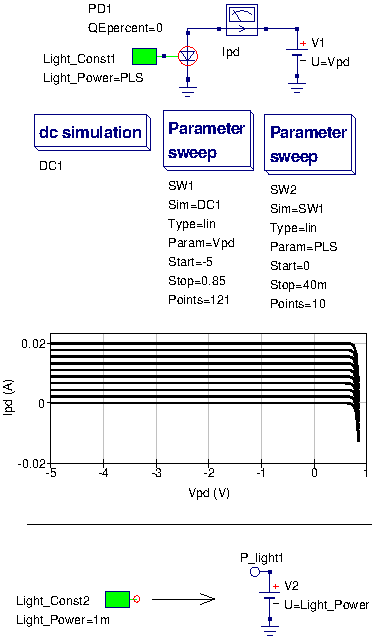
\includegraphics[width=0.55\linewidth]{PD_fig2}
        \caption{Basic photodiode test circuit for simulating device output current as a function of light input level and applied DC bias  }
  \label{fig:PD2}
\end{figure} 

\begin{figure}
  \centering
	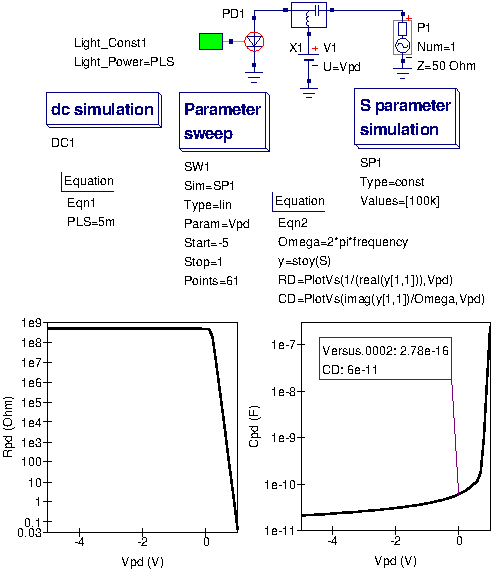
\includegraphics[width=0.8\linewidth]{PD_fig3}
        \caption{Photodiode test circuit for extracting device capacitance and resistance as a function of applied DC bias  }
  \label{fig:PD3}
\end{figure} 

\begin{figure} 
  \centering
	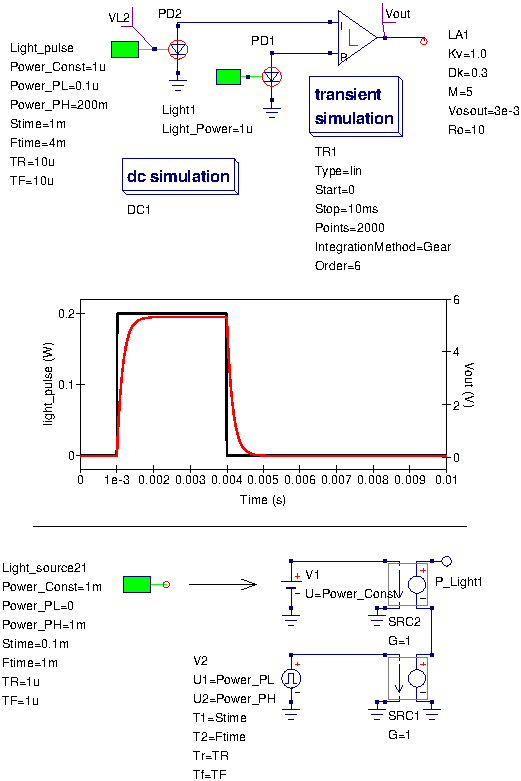
\includegraphics[width=0.8\linewidth]{PD_fig4}
        \caption{Pulsed light power comparator circuit using two photodiodes and a logarithmic amplifier  }
  \label{fig:PD4}
\end{figure} 

\begin{figure}
  \centering
	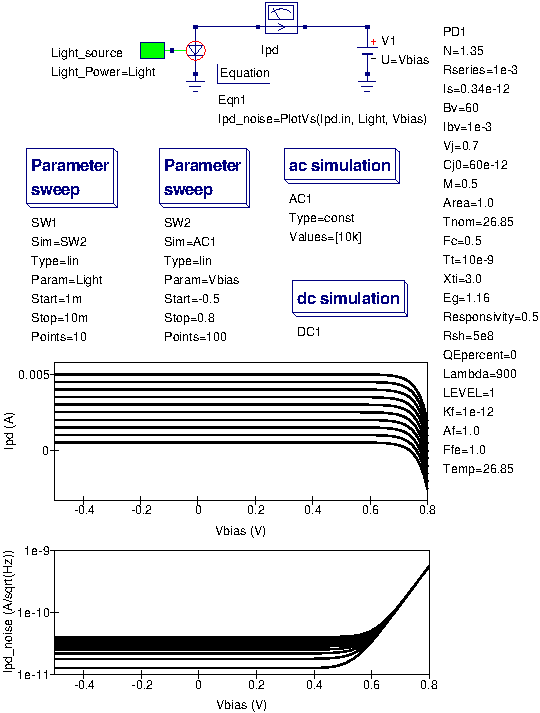
\includegraphics[width=0.8\linewidth]{PD_fig5}
        \caption{Photodiode noise test circuit and simulated noise characteristics  }
  \label{fig:PD5}
\end{figure} 



\tutsection{End Note}

Optoelectronic devices are an important group of electronic components
and as such deserve more attention than has been given to them in the
past by the Qucs development team.  This situation should improve over
the coming year. The pn junction photodiode model is the first in a
planned series of optoelectronic models, including models for
transimpedance amplifiers, optical actuators and optical media. Given
time it should be possible to significantly improve Qucs
optoelectronic capabilities.  The photodiode model reported here is an
interesting model in that it is one of the first Verilog-A models to
fully utilize the recent changes to the ADMS/Qucs interface which
allow proper initialisation of model parameters. A new procedure for
combining Verilog-A generated models also introduces for the first
time the initial stages towards a fully modularized approach to
linking complex models with the main body of the Qucs code.  Once
again my thanks to Stefan Jahn for all his encouragement and help
during the period I worked on the photodiode model.



